\section{Implementation}

This chapter describes the implementation of methods for each iteration's interactions: in regards to data, data analysis, method, and method analysis. Figure \ref{fig:iterative-process} is made to assist the reader in which methods were used for each iteration, in terms of research and app tests.

%study design, application development, and for data analysis theory.

\begin{figure}[h]
    \centering
    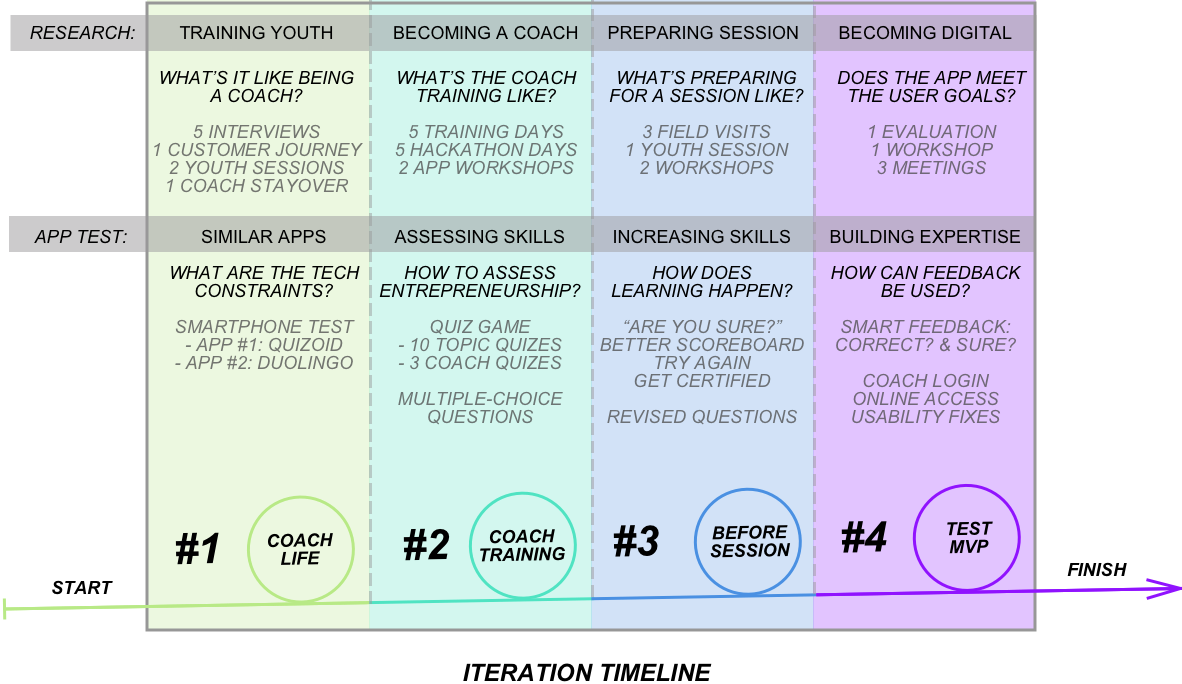
\includegraphics[width=1.0\textwidth]{iterativeProcess.png}
    \caption{The iteration timeline shows the process from iteration 1-4, by different colors. Each iteration leads to a loop, with the design situation as the focus, in which interactions can happen that is related to either research ("What's ...?") and an app test ("How can we ...?"). This output from the loop, then gives force to the next iteration.}
    \label{fig:iterative-process}
\end{figure}

Methods w/ Analysis
----

5 Interviews - Notes - Questionnaire for Customer Journey
1 Customer Journey - Clustering - Personas
2 Youth Sessions - Shadowing - Needs
1 Coach Stayover - Empathy - Design Ethnography

5 Training Days - Observations - Understanding entrepreneurship training
5 Hackathon Days - Interviews - Notes and Sketches
2 App Workshops - Co-Creation/Co-Refinement - Sketches and Needs

3 Field

Acitivity
App test observations (group)

App test observation (individual)
- Affective reactions (5 Why's, think aloud)

Analysis: Interaction design evaluation (desirability, usability, utility, pleasurability)

Customer Journey Map
- Activities
- Behaviour

Written responses (individual)
- Right/wrong
- Time
- Number of tries

Interviews
- New insights

Data Collection w/ Analysis
----

Customer Journey Map w/ clustering

Pre-study w/ Quantative analysis

Written quiz responses w/ Quantative analysis

Digital quiz responses / Quantative analysis + Statistical analysis + Parallell coordinates

Quiz questions 1 w/ Bloom analysis
Quiz questions 2 w/ Bloom analysis

%\input{implementation/iteration-1}

%\input{implementation/iteration-2}

%\input{implementation/iteration-3}

%\input{implementation/iteration-4}
